\documentclass[12pt]{beamer}
\usepackage{../Estilos/BeamerMAF}
\usepackage{arydshln}
%Sección para el tema de beamer, con el theme, usercolortheme y sección de footers
\usetheme{Frankfurt}
\usecolortheme{beaver}
%\useoutertheme{default}
\setbeamercovered{invisible}
% or whatever (possibly just delete it)
\setbeamertemplate{section in toc}[sections numbered]
\setbeamertemplate{subsection in toc}[subsections numbered]
\setbeamertemplate{subsection in toc}{\leavevmode\leftskip=3.2em\rlap{\hskip-2em\inserttocsectionnumber.\inserttocsubsectionnumber}\inserttocsubsection\par}
% \setbeamercolor{section in toc}{fg=blue}
% \setbeamercolor{subsection in toc}{fg=blue}
% \setbeamercolor{frametitle}{fg=blue}
\setbeamertemplate{caption}[numbered]

\setbeamertemplate{footline}
\beamertemplatenavigationsymbolsempty
\setbeamertemplate{headline}{}


\makeatletter
% \setbeamercolor{section in foot}{bg=gray!30, fg=black!90!orange}
% \setbeamercolor{subsection in foot}{bg=blue!30!yellow, fg=red}
% \setbeamercolor{date in foot}{bg=black, fg=white}
\setbeamertemplate{footline}
{
  \leavevmode%
  \hbox{%
  \begin{beamercolorbox}[wd=.333333\paperwidth,ht=2.25ex,dp=1ex,center]{section in foot}%
    \usebeamerfont{section in foot} \insertsection
  \end{beamercolorbox}%
  \begin{beamercolorbox}[wd=.333333\paperwidth,ht=2.25ex,dp=1ex,center]{subsection in foot}%
    \usebeamerfont{subsection in foot}  \insertsubsection
  \end{beamercolorbox}%
  \begin{beamercolorbox}[wd=.333333\paperwidth,ht=2.25ex,dp=1ex,right]{date in head/foot}%
    \usebeamerfont{date in head/foot} \insertshortdate{} \hspace*{2em}
    \insertframenumber{} / \inserttotalframenumber \hspace*{2ex} 
  \end{beamercolorbox}}%
  \vskip0pt%
}







\title{\large{Propiedades de los armónicos esféricos}}
\subtitle{Tema 4}

\author{M. en C. Gustavo Contreras Mayén}
\date{24 de noviembre de 2021}

\begin{document}
\maketitle
\fontsize{14}{14}\selectfont
\spanishdecimal{.}

\section*{Contenido}
\frame[allowframebreaks]{\tableofcontents[currentsection, hideallsubsections]}

%Ref. Zettili (2009) 5.7 Properties of the Spherical Harmonics
\section{Propiedades de los Armónicos esféricos}
\frame{\tableofcontents[currentsection, hideothersubsections]}
\subsection{Forman una base completa}

\begin{frame}
\frametitle{Los $Y_{lm} (\theta, \varphi)$ como funciones propias}
Los $Y_{lm} (\theta, \varphi)$ son funciones propias de los operadores $\vb{L}^{2}$ y de $L_{z}$, \pause son ortonormales:
\pause
\begin{align*}
\setlength{\fboxsep}{3\fboxsep}\boxed{
\scaleint{5ex}_{\bs 0}^{2 \pi} \scaleint{5ex}_{\bs 0}^{\pi} \sin \theta Y_{\pderivada{l} \pderivada{m}}^{*} (\theta, \varphi) Y_{lm} (\theta, \varphi) \dd{\theta} \dd{\varphi} = \delta_{\pderivada{l} l} \, \delta_{\pderivada{m} m} }
\end{align*}
\end{frame}
\begin{frame}
\frametitle{Base completa}
Por lo que forman una base ortonormal en el espacio de Hilbert de las funciones de cuadrado integrable para $\theta$ y $\varphi$.
\end{frame}
\begin{frame}
\frametitle{Base completa}
La relación de completitud (o cerradura) está dada por:
\pause
\begin{align*}
\nsum_{-l}^{l} \ket{l, m} \bra{l, m} = 1
\end{align*}
\end{frame}
\begin{frame}
\frametitle{Base completa}
De manera equivalente:
\pause
\begin{eqnarray*}
\begin{aligned}
\nsum_{m} \ip{\theta \varphi}{l, m} \ip{l, m}{\pderivada{\theta} \pderivada{\varphi}} &= \pause \nsum_{m} Y_{lm}^{*} (\pderivada{\theta}, \pderivada{\varphi}) Y_{lm} (\theta, \varphi) = \\[0.5em] \pause
&= \delta (\cos \theta - \cos \pderivada{\theta}) \, \delta (\varphi - \pderivada{\varphi}) = \\[0.5em] \pause
&= \dfrac{\delta (\theta - \pderivada{\theta})}{\sin \theta} \, \delta (\varphi - \pderivada{\varphi})
\end{aligned}
\end{eqnarray*}
\end{frame}

\subsection{Su relación con los \texorpdfstring{$P_{l}^{m}(\cos \theta)$}{Plm (cos t)}}

\begin{frame}
\frametitle{Relación con los Polinomios asociados de Legendre}
Los armónicos esféricos están relacionados con los polinomios asociados de Legendre $P_{l}^{m}(\cos \theta)$ de la siguiente manera:
\pause
\begin{align*}
Y_{lm}(\theta, \varphi) {=} (-1)^{m} \sqrt{\bigg( \dfrac{ 2 l {+} 1}{4 \pi} \bigg)\bigg( \dfrac{(l {-} m)!}{(l {+} m)!} \bigg)} P_{l}^{m} (\cos \theta) e^{i m \varphi}
\end{align*}
con $m \geq 0$.
\end{frame}

\subsection{Son funciones complejas}

\begin{frame}
\frametitle{Complejo conjugado}
Los armónicos esféricos son funciones complejas, \pause por lo que su conjugado complejo está dado por:
\begin{align*}
\setlength{\fboxsep}{3\fboxsep}\boxed{
\bigg[ Y_{lm} (\theta, \varphi) \bigg]^{*} = (-1)^{m} \, Y_{l, -m} (\theta, \varphi) }
\end{align*}
\end{frame}

\subsection{Funciones propias del operador de paridad}

\begin{frame}
\frametitle{El operador de paridad}
Se puede demostrar que $Y_{lm} (\theta, \varphi)$ es un estado propio del operador de paridad $\hat{P}$, con un valor propio $(-1)^{l}$:
\pause
\begin{align*}
\setlength{\fboxsep}{3\fboxsep}\boxed{
\hat{P} \, Y_{lm}(\theta, \varphi) = Y_{lm} (\pi {-} \theta, \varphi {+} \pi) = (-1)^{l} \, Y_{lm}(\theta, \varphi)}
\end{align*}
\end{frame}
\begin{frame}
\frametitle{Reflexión sobre el origen}
Para una reflexión espacial alrededor del origen $\va*{r}^{\, \prime} = - \va{r}$, corresponde entonces:
\pause
\setbeamercolor{item projected}{bg=blue!70!black,fg=yellow}
\setbeamertemplate{enumerate items}[circle]
\begin{enumerate}[<+->]
\item $\pderivada{r} = r$
\item $\pderivada{\theta} = \pi - \theta$
\item $\pderivada{\varphi} = \pi + \varphi$
\end{enumerate}
\end{frame}
\begin{frame}
\frametitle{Usando propiedades de los $P_{l}^{m}(\cos \theta)$}
Que al utilizar de manera adelantada una de los propiedades de los polinomios asociados de Legendre, se tiene que:
\pause
\begin{eqnarray*}
P_{l}^{m} (\cos \pderivada{\theta}) = \pause P_{l}^{m} (- \cos \theta) = \pause (-1)^{l+m} \, P_{l}^{m} (\cos \theta)
\end{eqnarray*}
\pause
Y por último:
\pause
\begin{eqnarray*}
e^{i m \pderivada{\varphi}} = \pause e^{i m \pi} e^{i m \varphi} = \pause (-1)^{m} \, e^{i m \varphi}
\end{eqnarray*}
\end{frame}

\subsection{Su relación con los \texorpdfstring{$P_{l}(\cos \theta)$}{Pl(cos t)}.}

\begin{frame}
\frametitle{Los $Y_{lm}$ y los $P_{l}(\cos \theta)$}
Se establece una conexión entre los armónicos esféricos y los polinomios ordinarios de Legendre, haciendo que $m = 0$ en la ecuación:
\pause
\begin{align*}
&Y_{lm}(\theta, \varphi) {=} \dfrac{(-1)^{l}}{2^{l} l!} \sqrt{\bigg( \dfrac{ 2 l {+} 1}{4 \pi} \bigg)\bigg( \dfrac{(l {-} m)!}{(l {+} m)!} \bigg)} e^{i m \varphi} \times \\[0.5em]
&\times \dfrac{1}{\sin^{m} \theta} \, \dv[l-m]{(\cos \theta)} \, (\sin \theta)^{2l}
\end{align*}
\end{frame}
\begin{frame}
\frametitle{Lo que nos lleva a}
Entonces, con $m = 0$, se tiene:
\pause
\begin{eqnarray*}
\begin{aligned}
Y_{l0}(\theta, \varphi) &= \dfrac{(-1)^{l}}{2^{l} l!} \sqrt{ \dfrac{ 2 l {+} 1}{4 \pi}} \, \dv[l]{(\cos \theta)} \, (\sin \theta)^{2l} = \\[0.5em] \pause
&= \sqrt{ \dfrac{ 2 l {+} 1}{4 \pi}} \, P_{l} (\cos \theta)
\end{aligned}
\end{eqnarray*}
\pause
donde:
\pause
\begin{align*}
P_{l} (\cos \theta) = \dfrac{(-1)^{l}}{2^{l} l!} \, \dv[l]{(\cos \theta)} \, (\cos^{2} \theta - 1)^{l}
\end{align*}
\end{frame}
\begin{frame}
\frametitle{Resultado interesante}
De la expresión para los $Y_{lm}$, se puede verificar que:
\pause
\begin{align*}
Y_{lm} (0, \varphi) = \sqrt{\dfrac{2 \, l + 1}{4 \, \pi}} \, \delta_{m, 0}
\end{align*}
\end{frame}
\begin{frame}
\frametitle{Tabla de algunos $Y_{lm}(\theta, \varphi)$}
\begin{eqnarray*}
\begin{aligned}
Y_{00} (\theta, \varphi) &= \dfrac{1}{\sqrt{4 \, \pi}} \\[0.5em] \pause
Y_{10} (\theta, \varphi) &= \sqrt{\dfrac{3}{4 \, \pi}} \, \cos \theta \\[0.5em] \pause
Y_{1, \pm 1} (\theta, \varphi) &= \mp \sqrt{\dfrac{3}{8 \, \pi}} \, e^{\pm i \varphi} \sin \theta
\end{aligned}
\end{eqnarray*}
\end{frame}    
\begin{frame}
\frametitle{Tabla de algunos $Y_{lm}(\theta, \varphi)$}
\begin{eqnarray*}
\begin{aligned}
Y_{20} (\theta, \varphi) &= \sqrt{\dfrac{5}{16 \, \pi}} (3 \, \cos^{2} \theta - 1) \\[0.5em] \pause
Y_{2, \pm 1} (\theta, \varphi) &= \mp \sqrt{\dfrac{15}{8 \, \pi}} \, e^{\pm i \varphi} \sin \theta \, \cos \theta \\[0.5em] \pause
Y_{2, \pm 2} (\theta, \varphi) &= \mp \dfrac{15}{\sqrt{32 \, \pi}} \, e^{\pm 2 i \varphi} \sin^{2} \theta
\end{aligned}
\end{eqnarray*}
\end{frame}
\begin{frame}
\frametitle{Gráfica de $\abs{Y_{0}^{0} (\theta, \varphi)}^{2}$}
\begin{figure}
    \centering
    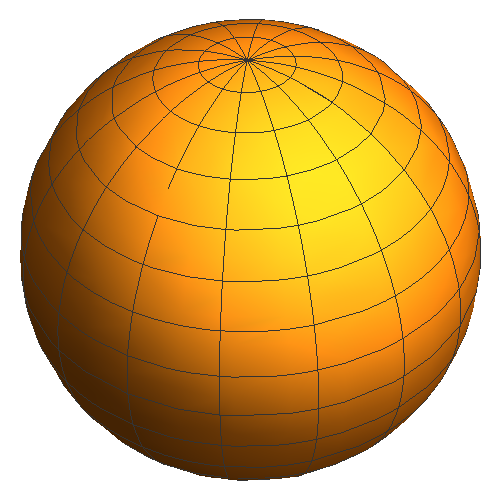
\includegraphics[scale=0.8]{Imagenes/AE2_00.eps}
\end{figure}
\end{frame}
\begin{frame}
\frametitle{Gráfica de $\abs{Y_{1}^{0} (\theta, \varphi)}^{2}$}
\begin{figure}
    \centering
    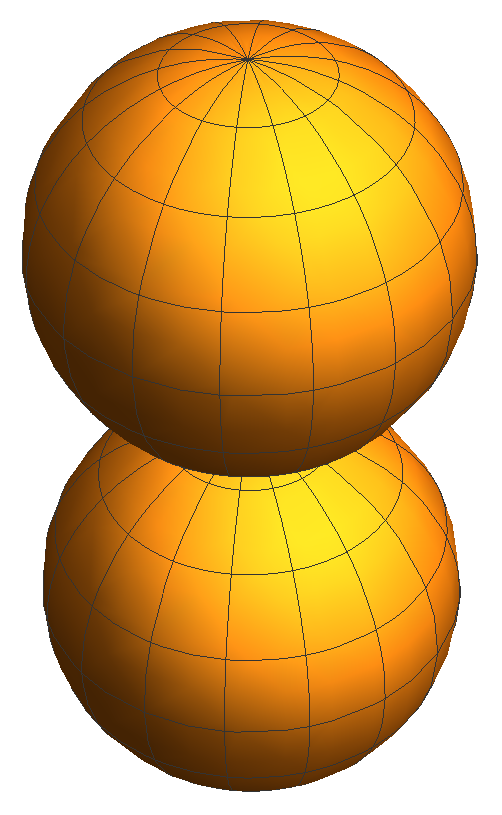
\includegraphics[scale=0.5]{Imagenes/AE2_10.eps}
\end{figure}
\end{frame}
\begin{frame}
\frametitle{Gráfica de $\abs{Y_{1}^{\pm 1} (\theta, \varphi)}^{2}$}
\begin{figure}
    \centering
    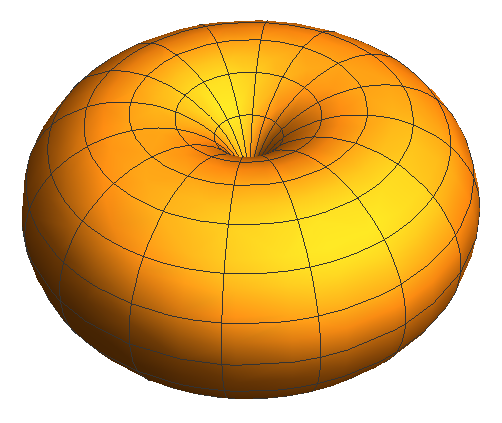
\includegraphics[scale=0.8]{Imagenes/AE2_11.eps}
\end{figure}
\end{frame}
\begin{frame}
\frametitle{Gráfica de $\abs{Y_{2}^{0} (\theta, \varphi)}^{2}$}
\begin{figure}
    \centering
    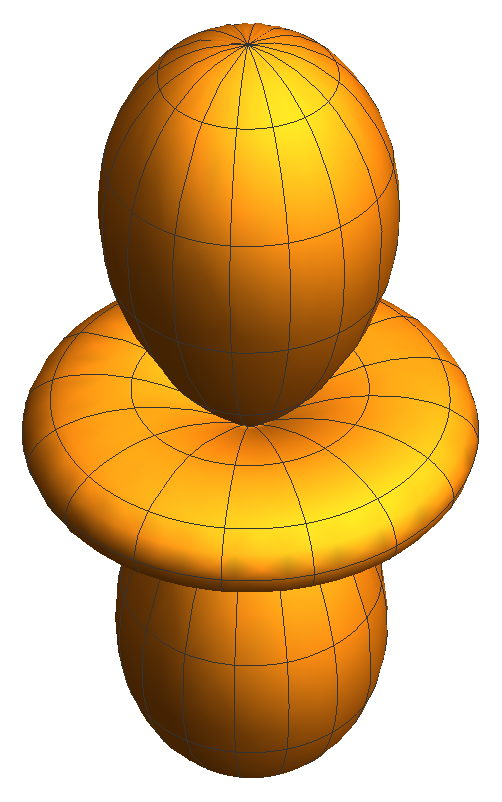
\includegraphics[scale=0.5]{Imagenes/AE2_20.eps}
\end{figure}
\end{frame}
\begin{frame}
\frametitle{Gráfica de $\abs{Y_{2}^{\pm 1} (\theta, \varphi)}^{2}$}
\begin{figure}
    \centering
    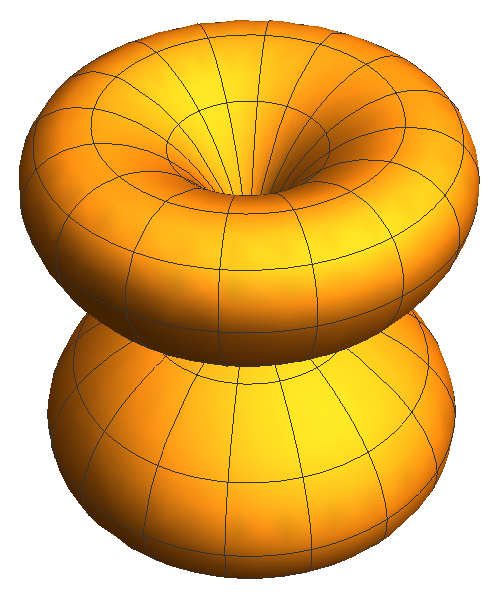
\includegraphics[scale=0.75]{Imagenes/AE2_21.eps}
\end{figure}
\end{frame}
\begin{frame}
\frametitle{Gráfica de $\abs{Y_{2}^{\pm 2} (\theta, \varphi)}^{2}$}
\begin{figure}
    \centering
    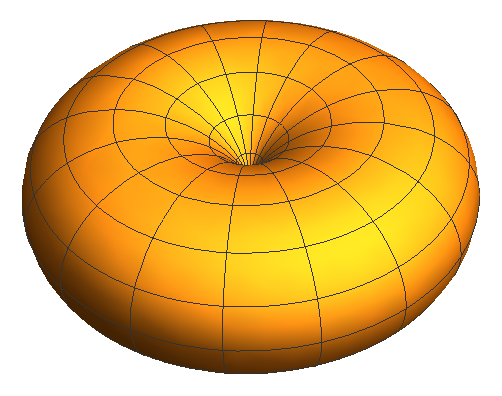
\includegraphics[scale=0.8]{Imagenes/AE2_22.eps}
\end{figure}
\end{frame}
\begin{frame}
\frametitle{Gráfica en el espacio angular}
La gráfica esférica visualiza la forma del $Y_{lm}(\theta, \varphi)$ en un espacio angular.
\\
\bigskip
\pause
La distancia de la superficie del origen a valores $\theta, \varphi$ dados, es la función que se grafica. \pause El valor absoluto elimina la dependencia de $\varphi$, por lo que solo se ve la dependencia $\theta$.
\end{frame}
\begin{frame}
\frametitle{Parte real o imaginaria}
Para ver la dependencia de $\varphi$ se puede tomar ya sea la parte real o la imaginaria.
\\
\bigskip
\pause
Como se verá a continuación:
\end{frame}
\begin{frame}
\frametitle{Gráfica de $\Re{Y_{2}^{0} (\theta, \varphi)}$}
\begin{figure}
    \centering
    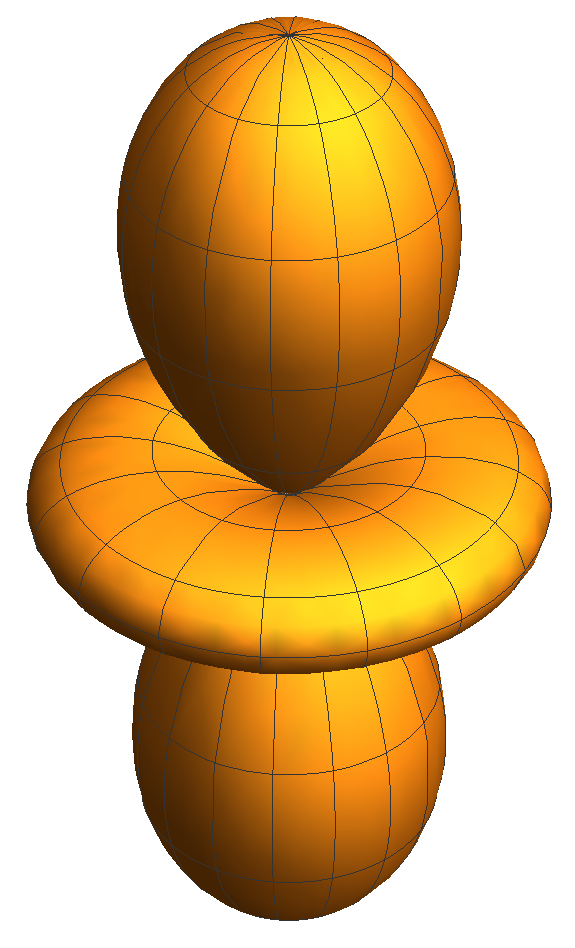
\includegraphics[scale=0.45]{Imagenes/AE_Re_20.eps}
\end{figure}
\end{frame}
\begin{frame}
\frametitle{Gráfica de $\Re{Y_{2}^{1} (\theta, \varphi)}$}
\begin{figure}
    \centering
    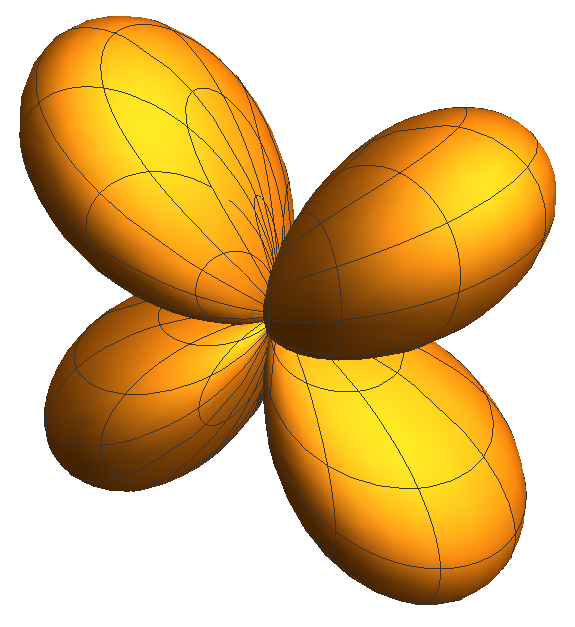
\includegraphics[scale=0.7]{Imagenes/AE_Re_21.eps}
\end{figure}
\end{frame}
\begin{frame}
\frametitle{Gráfica de $\Re{Y_{2}^{2} (\theta, \varphi)}$}
\begin{figure}
    \centering
    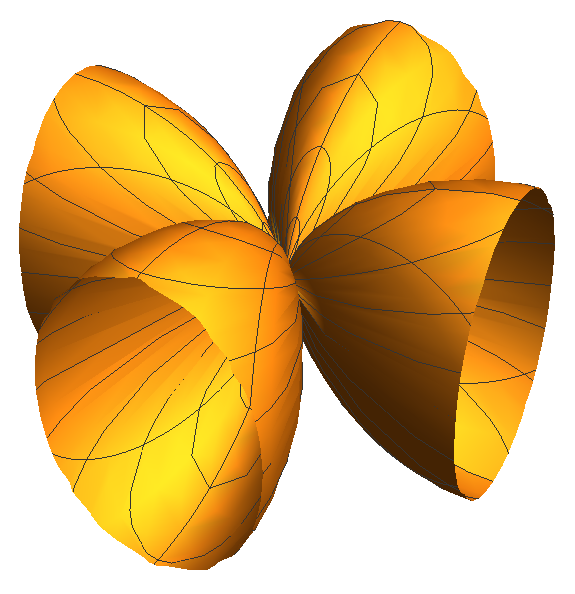
\includegraphics[scale=0.75]{Imagenes/AE_Re_22.eps}
\end{figure}
\end{frame}

\section{Ejercicio con los \texorpdfstring{$Y_{lm}(\theta, \varphi)$}{Ylm (t,f)}}
\frame{\tableofcontents[currentsection, hideothersubsections]}
\subsection{Uso de los operadores escalera}

\begin{frame}
\frametitle{Enunciado del ejercicio}
\setbeamercolor{item projected}{bg=blue!70!black,fg=yellow}
\setbeamertemplate{enumerate items}[circle]
\begin{enumerate}[<+->]
\item Usando la relación:
\begin{align*}
Y_{l0}(\theta, \varphi) = \sqrt{\dfrac{2 \, l + 1}{4 \, \pi}} \, P_{l} (\cos \theta)
\end{align*}
encuentra la expresión de $Y_{30}(\theta, \varphi)$
\item Usa la expresión $Y_{30}(\theta, \varphi)$ para inferir cuáles serán las de $Y_{3 \pm 1}(\theta, \varphi)$
\end{enumerate}
\end{frame}
\begin{frame}
\frametitle{Resolviendo el inciso $1)$}
Ya que $l = 3$, tomamos prestado el valor polinomio ordinario de Legendre $P_{3}(\cos \theta)$:
\pause
\begin{align*}
P_{3}(\cos \theta) = \dfrac{1}{2} \big( 5 \, \cos^{3} \theta - 3 \, \cos \theta \big)
\end{align*}
\end{frame}
\begin{frame}
\frametitle{Calculando el $Y_{3 0}(\theta, \varphi)$}
Por lo que se tendrá:
\begin{eqnarray*}
\begin{aligned}
Y_{3 0}(\theta, \varphi) &= \sqrt{\dfrac{2 \, l + 1}{4 \, \pi}} \, P_{3}(\cos \theta) \\[0.5em] \pause
&= - 3 \hbar \sqrt{\dfrac{7}{16 \, \pi}} \big( 5 \, \cos^{3} \theta - 3 \, \cos \theta \big)
\end{aligned}
\end{eqnarray*}
\end{frame}
\begin{frame}
\frametitle{Resolviendo el inciso $2)$}
Para calcular el $Y_{31}$ a partir del $Y_{30}$ \pause se necesita aplicar el operador de ascenso $L_{+}$ sobre $Y_{30}$ en dos momentos: \pause inicialmente de manera algebraica:
\pause
\begin{eqnarray*}
\begin{aligned}
L_{+} \, Y_{30} &= \hbar \, \sqrt{3 (3 + 1)- 0} \, Y_{31} \\[0.5em] \pause
&= 2 \, \hbar \sqrt{3} \, Y_{31}
\end{aligned}
\end{eqnarray*}
\pause
Por lo tanto:
\pause
\begin{align*}
Y_{31} = \dfrac{1}{2 \, \hbar \sqrt{3}} \, L_{+} \, Y_{30}
\end{align*}
\end{frame}
\begin{frame}
\frametitle{Resolviendo el inciso $2)$}
Ahora usamos la forma diferencial de $L_{+}$:
\pause
\begin{eqnarray*}
\begin{aligned}
&L_{+} \, Y_{30} (\theta, \varphi) = \hbar \, e^{i \varphi} \bigg[ \pdv{\theta} + i \, \dfrac{\cos \theta}{\sin \theta} \pdv{\varphi} \bigg] Y_{30} (\theta, \varphi) = \\[0.5em] \pause
&= \hbar \sqrt{\dfrac{7}{16 \pi}} e^{i \varphi} \bigg[ \pdv{\theta} + i \, \dfrac{\cos \theta}{\sin \theta} \pdv{\varphi} \bigg] \big( 5 \cos^{3} \theta {-} 3 \cos \theta \big) = \\[0.5em] \pause 
&= - 3 \hbar \sqrt{\dfrac{7}{16 \pi}} \, \sin \theta \big( 5 \, \cos^{2} - 1 \big) e^{i \varphi}
\end{aligned}
\end{eqnarray*}
\end{frame}
\begin{frame}
\frametitle{Resolviendo el inciso $2)$}
Sustituimos este resultado para obtener:
\pause
\begin{eqnarray*}
Y_{31} = \dfrac{1}{2 \, \hbar \sqrt{3}} \, L_{+} \, Y_{30} = \pause - \sqrt{\dfrac{21}{64 \pi}} \, \sin \theta \big( 5 \, \cos^{2} - 1 \big) e^{i \varphi}
\end{eqnarray*}
\end{frame}
\begin{frame}
\frametitle{Para calcular el $Y_{3,-1}$}
Para calcular el $Y_{3,-1}$ a partir del $Y_{30}$ \pause se necesita aplicar el operador de descenso $L_{-}$ sobre $Y_{30}$ en dos momentos: \pause inicialmente de manera algebraica:
\pause
\begin{eqnarray*}
\begin{aligned}
L_{-} \, Y_{30} &= \hbar \, \sqrt{3 (3 + 1)- 0} \, Y_{3,-1} \\[0.5em] \pause
&= 2 \, \hbar \sqrt{3} \, Y_{3,-1}
\end{aligned}
\end{eqnarray*}
\pause
Por lo tanto:
\pause
\begin{align*}
Y_{3,-1} = \dfrac{1}{2 \, \hbar \sqrt{3}} \, L_{-} \, Y_{30}
\end{align*}
\end{frame}
\begin{frame}
\frametitle{Para calcular el $Y_{3,-1}$}
Ahora usamos la forma diferencial de $L_{-}$:
\pause
\begin{eqnarray*}
\begin{aligned}
&L_{-} \, Y_{30} (\theta, \varphi) = - \hbar \, e^{i \varphi} \bigg[ \pdv{\theta} - i \, \dfrac{\cos \theta}{\sin \theta} \pdv{\varphi} \bigg] Y_{30} (\theta, \varphi) = \\[0.5em] \pause
&= - \hbar \sqrt{\dfrac{7}{16 \pi}} e^{i \varphi} \bigg[ \pdv{\theta} - i \, \dfrac{\cos \theta}{\sin \theta} \pdv{\varphi} \bigg] \big( 5 \cos^{3} \theta {-} 3 \cos \theta \big) = \\[0.5em] \pause 
&= 3\hbar \sqrt{\dfrac{7}{16 \pi}} \, \sin \theta \big( 5 \, \cos^{2} - 1 \big) e^{-i \varphi}
\end{aligned}
\end{eqnarray*}
\end{frame}
\begin{frame}
\frametitle{Para calcular el $Y_{3,-1}$}
Sustituimos este resultado para obtener:
\pause
\begin{eqnarray*}
Y_{3,-1} = \dfrac{1}{2 \, \hbar \sqrt{3}} \, L_{-} \, Y_{30} = \pause \sqrt{\dfrac{21}{64 \pi}} \, \sin \theta \big( 5 \, \cos^{2} - 1 \big) e^{-i \varphi}
\end{eqnarray*}
\end{frame}    
\end{document}